\documentclass[border=5pt]{standalone}
\usepackage{tikz}
\usepackage{xcolor}

\definecolor{danger}{RGB}{220,53,69}
\definecolor{warning}{RGB}{255,193,7}
\definecolor{secondary}{RGB}{108,117,125}
\definecolor{success}{RGB}{40,167,69}

\begin{document}
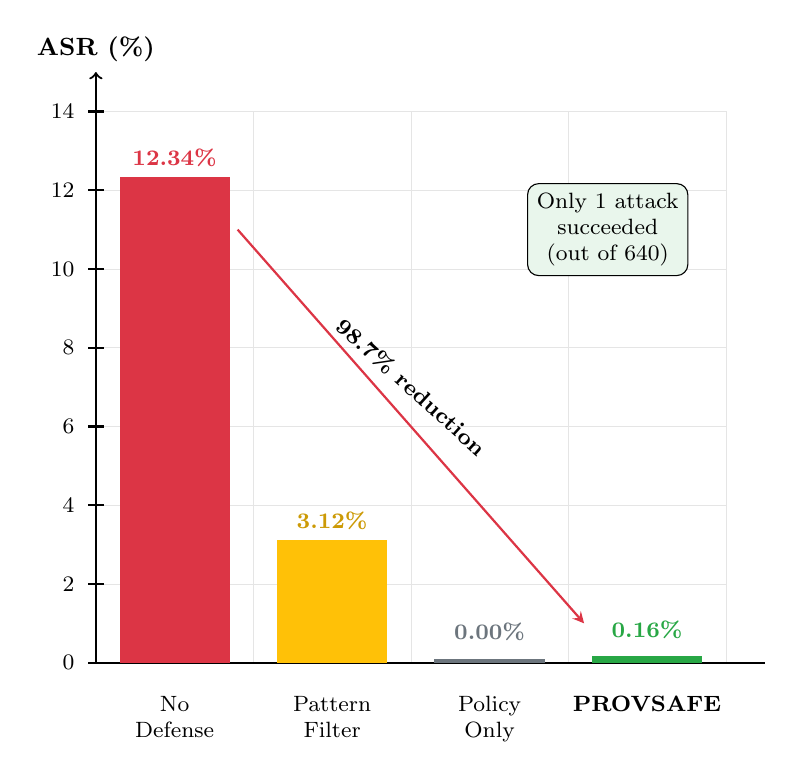
\begin{tikzpicture}[scale=1]
  % Background grid
  \draw[gray!20, very thin] (0,0) grid[xstep=2, ystep=1] (8,7);
  
  % Y-axis (ASR %)
  \draw[thick, ->] (0,0) -- (0,7.5) node[above, font=\small\bfseries] {ASR (\%)};
  \foreach \y/\label in {0/0, 1/2, 2/4, 3/6, 4/8, 5/10, 6/12, 7/14} {
    \draw[thick] (-0.1,\y) -- (0.1,\y);
    \node[left, font=\footnotesize] at (-0.15,\y) {\label};
  }
  
  % X-axis
  \draw[thick] (0,0) -- (8.5,0);
  
  % Bar positions and widths
  \def\barwidth{1.4}
  
  % No Defense: 12.34% ASR -> 12.34/2 = 6.17
  \fill[danger] (1-\barwidth/2, 0) rectangle (1+\barwidth/2, 6.17);
  \node[below, font=\footnotesize, align=center] at (1, -0.3) {No\\Defense};
  \node[above, font=\footnotesize\bfseries, danger] at (1, 6.17) {12.34\%};
  
  % Pattern Filter: 3.12% ASR -> 3.12/2 = 1.56
  \fill[warning] (3-\barwidth/2, 0) rectangle (3+\barwidth/2, 1.56);
  \node[below, font=\footnotesize, align=center] at (3, -0.3) {Pattern\\Filter};
  \node[above, font=\footnotesize\bfseries, warning!80!black] at (3, 1.56) {3.12\%};
  
  % Policy-Only: 0% ASR
  \fill[secondary] (5-\barwidth/2, 0) rectangle (5+\barwidth/2, 0.05);
  \node[below, font=\footnotesize, align=center] at (5, -0.3) {Policy\\Only};
  \node[above, font=\footnotesize\bfseries, secondary] at (5, 0.15) {0.00\%};
  
  % PROVSAFE: 0.16% ASR -> 0.16/2 = 0.08
  \fill[success] (7-\barwidth/2, 0) rectangle (7+\barwidth/2, 0.08);
  \node[below, font=\footnotesize, align=center] at (7, -0.3) {\textbf{PROVSAFE}};
  \node[above, font=\footnotesize\bfseries, success] at (7, 0.18) {\textbf{0.16\%}};
  
  % Reduction arrow
  \draw[thick, ->, >=stealth, danger] (1.8, 5.5) -- (6.2, 0.5);
  \node[font=\footnotesize, rotate=-42] at (4, 3.5) {\textbf{98.7\% reduction}};
  
  % Legend annotation
  \node[draw, rounded corners, fill=success!10, font=\footnotesize, align=center] 
    at (6.5, 5.5) {Only 1 attack\\succeeded\\(out of 640)};
  
\end{tikzpicture}
\end{document}
